Formally, we define graph constraints via the notion of (nested) graph conditions according to \cite{DBLP:journals/mscs/HabelP09}.
Nested graph conditions provide the concepts for both, graph constraints and application conditions for graph transformation rules.
Conditions are called constraints in the context of graphs where conditions may globally restrict the structure of graphs and are called application conditions in the context of rule definitions where conditions may restrict the application of rules.
\index{graph constraint}\index{application condition}

\begin{definition}[(Nested) Condition and Satisfaction (Def. 2.7 \& 2.8 in \cite{FAGT2})]
\label{def:condition-satisfaction}
\emph{A (nested) condition $\ac_P$}\index{graph condition} over a premise object $P$ is inductively defined by:
%\vspace{-2ex}
\begin{itemize}
	\item $\true$ is a condition over $P$.
	\item For every morphism $(a \colon P \to C)$ and condition $\ac_C$ over $C$, $\exists(a,\ac_C)$ is a condition over $P$.
	Object $C$ is called the conclusion w.r.t. premise object $P$.
	\item Boolean formulae over conditions, i.e., $\neg\ac_P$, $\vee_{i \in I} (\ac_{P,i})$, $\wedge_{i \in I} (\ac_{P,i})$, are conditions over $P$ for conditions $\ac_P$ and $\ac_{P,i},(i \in I)$ over $P$ for some index set $I$.
\end{itemize}

\noindent
\emph{A morphism $p \colon P \to G$ satisfies a condition $\ac_P$ over $P$}\index{graph condition!"standard" satisfaction} (written $p \models \ac_P$), if $p \in \morO$ and:
\begin{itemize}
	\item $\ac_P = \true$, or
	\item $\ac_P = \exists(a \colon P \to C,\ac_C)$,  $\exists \ q \colon C \to G \in \M$ with $q \circ a = p$ and $q \models \ac_C$, or
	\item $\ac_P = \neg \ac'_P$ and $\neg (p \models \ac'_P)$, or
	\item $\ac_P = \wedge_{i \in I} (\ac_{P,i})$ and for all $i \in I$ it holds that $p \models \ac_{P,i}$, or 
	\item $\ac_P = \vee_{i \in I} (\ac_{P,i})$ and there is an $i \in I$ with $p \models \ac_{P,i}$.
\end{itemize}
Two conditions $\ac_P$ and $\ac'_P$ over $P$ are equivalent, written $\ac_P \equiv \ac'_P$, if for all morphisms $p\colon P \to G$ it is true that $p \models \ac_P$ if and only if $p \models \ac'_P$\index{graph condition!equivalence}.
In contrast to the standard satisfiability of conditions via $\models$, $\models_{\morO}$ defines the satisfiability of conditions with $q \in \morO$ instead of $q \in \M$ ($\morO$-satisfiability)\index{graph condition!$\morO$-satisfaction}.
For a nested condition $\ac_P$, the number of nestings is given by the largest number of sequenced morphisms in $\ac_P$.
If the number of nestings of $\ac_P$ is zero or one, then $\ac_P$ is called a plain condition \index{graph condition!plain}.
According to \cref{sec-gt-graphs,def:sec-gt-graphs:typed_graphs}, for a given type graph $\TG$, we say that a condition $\ac_P$ is typed over $\TG$, if all objects (graphs) in $\ac_P$ are typed over $\TG$\index{graph condition!typed over}.
Consequently, a set of conditions $C$ is typed over $\TG$, if all $\ac \in C$ are typed over $\TG$.
A condition $\ac_P$ is finite\index{graph condition!finite}, if the index set $I$ of every conjunction $\wedge_{i \in I}$ and disjunction $\vee_{i \in I}$ in $\ac_P$ is finite \cite{DBLP:journals/mscs/HabelP09}.
\envEndMarker
\end{definition}

\begin{remark}[Conditions -- Abbreviations]
Although not being explicitly defined in \cref{def:condition-satisfaction}, we use the following abbreviations for conditions: $\false:=\neg\true$, $\ac_P \Rightarrow \ac'_P:=\ac'_P \vee \neg\ac_P$, and $\ac_P \Leftrightarrow \ac'_P:=(\ac_P \Rightarrow \ac'_P) \wedge (\ac'_P \Rightarrow \ac_P)$.
\envEndMarker
\end{remark}

\begin{definition}[Positive Condition (Def 2.4 in \cite{DBLP:journals/corr/abs-1209-1436})]
\label{def:sec-gc-gc:cond_pos}
\emph{A condition $\ac_P$ over $P$ is positive}\index{graph condition!positive} if it does not contain negations $\neg$, i.e., $\ac_P$ is built up only by:
\begin{enumerate*}
\item $\true$,
\item $\exists(a,\ac_C)$, and
\item $\vee_{i \in I} (\wedge_{i \in I}) (\ac_{P,i})$ with $I \neq \varnothing$.
\envEndMarker
\end{enumerate*}
\end{definition}

\begin{definition}[$\M$-normal form (Def. 5 in \cite{DBLP:journals/mscs/HabelP09})]
A condition $\ac_P$ is in \emph{$\M$-normal form}\index{graph condition!$\M$-normal form}, if for all sub-conditions $\exists(a,\ac)$ of $\ac_P$, morphism $a$ is in $\M$.
\envEndMarker
\end{definition}

Graph constraints are conditions that are extended to conditions over the initial object $I$ when evaluating their satisfaction by graphs (cf. Def. 5.10 in \cite{FAGT2}).
In accordance with \cite{DBLP:journals/corr/abs-1209-1436}, we distinguish between initial and general satisfaction of graph constraints.
While initial satisfaction refers to the existential satisfaction, general satisfaction refers to the universal satisfaction of constraints.
Thus, a graph $G$ initially satisfies a constraint $\ac_P$ if premise $P$ occurs in $G$ such that $\ac_P$ holds.
In contrast, a graph $G$ generally satisfies a constraint $\ac_P$ if for all occurrences of premise $P$ in $G$ condition $\ac_P$ holds.

\begin{definition}[Constraint and Satisfaction]
\label{def:constr_sat}
Let $\ac_P$ be a condition over $P$.
\emph{An object $G$ initially satisfies a constraint $\ac_P$}\index{graph constraint!satisfaction!initial}, written $G \stackrel{I}{\models} \ac_P$, if the initial morphism $i_G\colon I \to G$ satisfies condition $\ac_I=\exists(i_P\colon I \to P,\ac_P)$ over initial object $I$ and initial morphism $i_P$.
\emph{An object $G$ generally satisfies a constraint $\ac_P$}\index{graph constraint!satisfaction!general}, written $G \models \ac_P$, if the initial morphism $i_G\colon I \to G$ satisfies condition $\ac_I=\neg\exists(i_P\colon I \to P,\neg\ac_P)$ over initial object $I$ and initial morphism $i_P$.
\emph{An object $G$ initially (generally) satisfies a set of constraints $C$}\index{graph constraint!satisfaction!set of constraints}, written $G \stackrel{I}{\models} C$ ($G \models C$) if $G \stackrel{I}{\models} ac$ ($G \models \ac$) for all $\ac \in C$.
\envEndMarker
\end{definition}

\begin{remark}[Initial \& General Satisfaction of Constraints]
\label{rem:sec-gc-gc:init_gen_sat}
Note that for general satisfaction, condition $\forall(i_P\colon I \to P,\ac_P)$ is equivalently expressed by $\neg\exists(i_P\colon I \to P,\neg\ac_P)$.
This allows us to speak of positive conditions $\ac_P$ in the sense of \cref{def:sec-gc-gc:cond_pos} in view of their general satisfaction by graphs in \cref{sec-dc-general-res} while the conditions that are actually used for evaluating their satisfaction are not positive.
Note that by the uniqueness of initial morphisms, for conditions $\ac_P$ over $P$ we have that:
\begin{enumerate}
  \item $G \stackrel{I}{\models} \ac_P \Leftrightarrow \exists p\colon P \to G \in \M$ such that $p \models \ac_P$, and
  \item $G \models \ac_P \Leftrightarrow \forall p\colon P \to G \in \M$ it holds that $p \models \ac_P$.
  \envEndMarker
\end{enumerate}
\end{remark}

\begin{figure}[!tb]
\begin{center}
\begin{tikzpicture}[]
\fill (0,0) node[inner sep=1pt] (A) {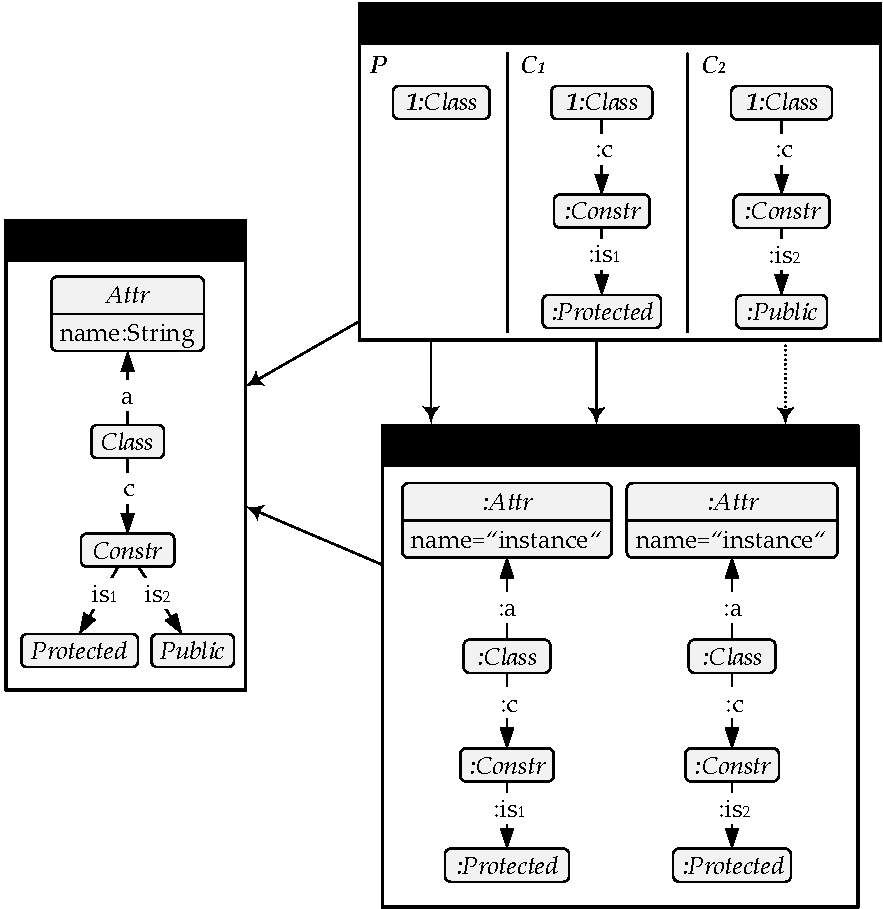
\includegraphics[width=.75\textwidth]{img/gen_intro/conditions.pdf}};
\fill (1.3,5.35) node[inner sep=1pt] (B) {\textcolor{white}{$\vee_{i=(1,2)}(\exists(a_i\colon P \to C_i,\true))$}};
\fill (-5.1,2.7) node[inner sep=1pt] (C) {\textcolor{white}{$\TG$}};
\fill (-.4,.125) node[inner sep=1pt] (D) {\textcolor{white}{$G$}};
\fill (-1.4,1.2) node[inner sep=1pt,fill=white] (E) {$t_P,t_{C_1},t_{C_2}$};
\fill (-.15,1) node[inner sep=1pt,fill=white] (F) {$p$};
\fill (2,1) node[inner sep=1pt,fill=white] (G) {$q_1$};
\fill (4.3,1) node[inner sep=1pt,fill=white] (H) {$q_2$};
\fill (-1.4,-1.1) node[inner sep=1pt,fill=white] (I) {$t_G$};
\end{tikzpicture}
\end{center}
\caption{Graph Constraints and their Satisfaction by Graphs}
\label{fig:sec-gc-gc:conditions}
\end{figure}

\begin{example}[Graph Constraint and Satisfaction]
In reference to the type graph $\TG_\CD$ of UML class diagrams in \cref{sec-gt-graphs,fig:sec-gt-graphs:atg}, \cref{fig:sec-gc-gc:conditions} depicts a modified type graph $\TG$, condition $\ac_P=\vee_{i=(1,2)}(\exists(a\colon P \to C_i,\true))$ over $P$ and graph $G$ both typed over $\TG$ via morphisms $(t_x\colon x \to \TG)_{x \in \{P,C_1,C_2,G\}}$.
According to type graph $\TG$, class diagrams may contain several \code{Class}es, each class may have several \code{Attr}ibutes each with a specific \code{name} of type \code{String} and each class has a \code{Constr}uctor with visibility \code{Protected} or \code{Public}.
Constraint $\ac_P$ claims that each class has a constructor with visibility protected or public.
Graph $G$ both initially and generally satisfies constraint $\ac_P$, since, morphism $p\colon P \to G \in \M$ can be mapped to the left or right class in $G$ such that there exists $q_1\colon C_1 \to G \in \M$ with $q_1 \circ a=p$ and $q_1 \models \true$.
However, there does not exist $q_2\colon C_2 \to G \in \M$ such that $q_2 \circ a=p$.
Thus, for constraint $\ac'_P=\wedge_{i=(1,2)}(\exists(a\colon P \to C_i,\true))$, $G$ satisfies $\ac'_P$ neither initially nor generally.
\envEndMarker
\end{example}

\paragraph*{Visual Notation}
According to \cref{par:sec-gt-graphs:vis}, the mapping of nodes, edges and attributes along morphisms correspond to their naming in visual notation.
For example in \cref{fig:sec-gc-gc:conditions}, node \code{:Class} in $P$ is mapped to node \code{:Class} in $C_1$ ($C_2$) along $a_1$ ($a_2$) as indicated by its name \code{1}.

\begin{figure}[!tb]
\begin{center}
\begin{tikzpicture}[]
\fill (0,0) node[inner sep=1pt] (A) {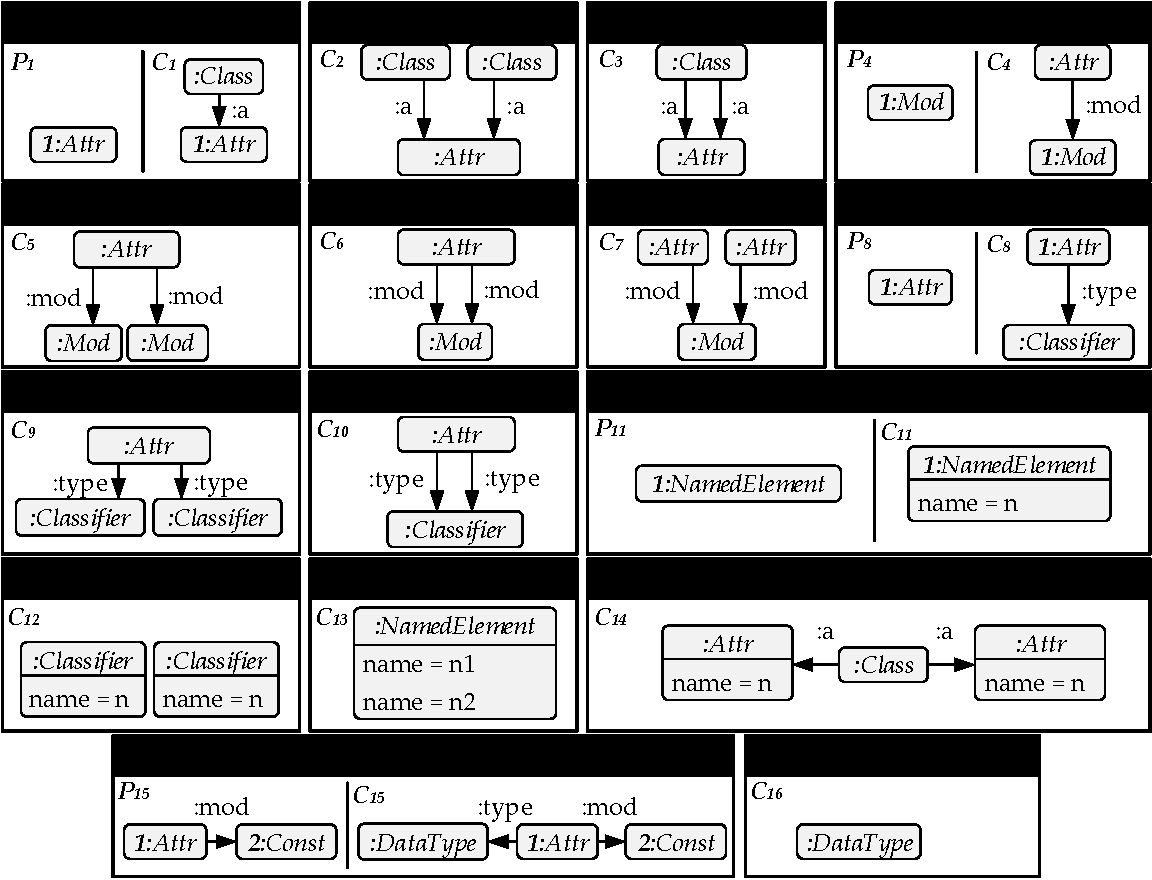
\includegraphics[width=\textwidth]{img/gen_intro/constraints.pdf}};
\fill (-5.8,5.35) node[inner sep=1pt] (B) {\textcolor{white}{$1|\exists(P_1 \to C_1,\true)$}};
\fill (-1.85,5.35) node[inner sep=1pt] (C) {\textcolor{white}{$2|\neg\exists(\varnothing \to C_2,\true)$}};
\fill (1.7,5.35) node[inner sep=1pt] (D) {\textcolor{white}{$3|\neg\exists(\varnothing \to C_3,\true)$}};
\fill (4.9,5.35) node[inner sep=1pt] (E) {\textcolor{white}{$4|\exists(P_4 \to C_4,\true)$}};
\fill (-5.8,3) node[inner sep=1pt] (B2) {\textcolor{white}{$5|\neg\exists(\varnothing \to C_5,\true)$}};
\fill (-1.85,3) node[inner sep=1pt] (C2) {\textcolor{white}{$6|\neg\exists(\varnothing \to C_6,\true)$}};
\fill (1.7,3) node[inner sep=1pt] (D2) {\textcolor{white}{$7|\neg\exists(\varnothing \to C_7,\true)$}};
\fill (4.9,3) node[inner sep=1pt] (E2) {\textcolor{white}{$8|\exists(P_8 \to C_8,\true)$}};
\fill (-5.8,.6) node[inner sep=1pt] (B3) {\textcolor{white}{$9|\neg\exists(\varnothing \to C_9,\true)$}};
\fill (-1.7,.6) node[inner sep=1pt] (C3) {\textcolor{white}{$10|\neg\exists(\varnothing \to C_{10},\true)$}};
\fill (1.85,.6) node[inner sep=1pt] (D3) {\textcolor{white}{$11|\exists(P_{11} \to C_{11},\true)$}};
\fill (-5.7,-1.8) node[inner sep=1pt] (B4) {\textcolor{white}{$12|\neg\exists(\varnothing \to C_{12},\true)$}};
\fill (-1.7,-1.8) node[inner sep=1pt] (C4) {\textcolor{white}{$13|\neg\exists(\varnothing \to C_{13},\true)$}};
\fill (1.85,-1.8) node[inner sep=1pt] (D4) {\textcolor{white}{$14|\neg\exists(\varnothing \to C_{14},\true)$}};
\fill (-4.2,-4.05) node[inner sep=1pt] (C5) {\textcolor{white}{$15|\exists(P_{15} \to C_{15},\true)$}};
\fill (3.75,-4.05) node[inner sep=1pt] (C16) {\textcolor{white}{$16|\exists(\varnothing \to C_{16},\true)$}};
\end{tikzpicture}
\end{center}
\caption{Graph Constraints for UML Class Diagrams}
\label{fig:sec-gc-gc:CD_constraints}
\label{fig:constraints2}
\end{figure}

\begin{example}[Graph Constraints for UML Class Diagrams]
\label{ex:sec-gc-gc:gc_UML_CD}
\cref{fig:sec-gc-gc:CD_constraints} depicts the graph constraints for UML class diagrams over type graph $\TG_\CD$ from \cref{sec-gt-graphs,fig:sec-gt-graphs:atg} which are used for verifying domain completeness in \cref{sec-dc-verification}.
All constraints in \cref{fig:sec-gc-gc:CD_constraints} are designated for general satisfaction.
According to \cref{sec-gt-graphs,ex:sec-gt-graph:type_graph}, this includes the multiplicity constraints in $\TG_\CD$ which complete the meta-model of UML class diagrams:
\begin{enumerate*}
\item Constraint \code{1} claims that each \code{Attr}ibute is assigned to a \code{Class} - in more detail - each attribute is assigned to exactly one class as refined by constraint \code{2},
\item Constraint \code{4} claims that each \code{Mod}ifier is the modifier of some attribute - in more detail - each modifier is the modifier of exactly one attribute as refined by constraint \code{7},
\item Analogously, constraint \code{8} claims that each attribute has some \code{type} - in more detail - each attribute has exactly one type as refined by constraint \code{9}, and
\item Constraint \code{5} claims that each attribute has zero or one modifier.
\end{enumerate*}
Beside the multiplicity constraints, the structure of class diagrams is additionally restricted by the following constraints:
\begin{enumerate*}
\item Constraints \code{3}, \code{6} and \code{10} forbid duplicate edges between two nodes,
\item Constraints \code{11} and \code{13} claim that each \code{NamedElement} has exactly one \code{name},
\item Constraint \code{12} claims that different \code{Classifiers} must have different names,
\item Constraint \code{14} claims that different attributes of the same class must have different names,
\item Constraint \code{15} claims that each \code{Const}ant attribute is of type \code{DataType} and not of type \code{Class}, and
\item Constraint \code{16} claims that there exists at least one \code{DataType}.
\end{enumerate*}
Note that according to \cref{sec-gt-graphs,rem:sec-gt-graphs:inheritance}, abstract node types \code{Mod}, \code{Classifier} and \code{NamedElement} are forbidden to be directly used in graphs like $P_4$.
However, instead of covering abstract types via the formal definition of graphs with node type inheritance, we assume dedicated constraints of the form $\vee_{s \in S}\exists(\code{1:t} \to \code{1:s},\true)$ for each abstract type $\code{t} \in \{\code{Mod},\code{Classifier},\code{NamedElement}\}$ and all non-abstract sub-types $S$ of \code{t} but that are not explicitly depicted in \cref{fig:sec-gc-gc:CD_constraints}.
\envEndMarker
\end{example}

\begin{figure}[!tb]
\begin{center}
\begin{tikzpicture}[]
\fill (0,0) node[inner sep=1pt] (A) {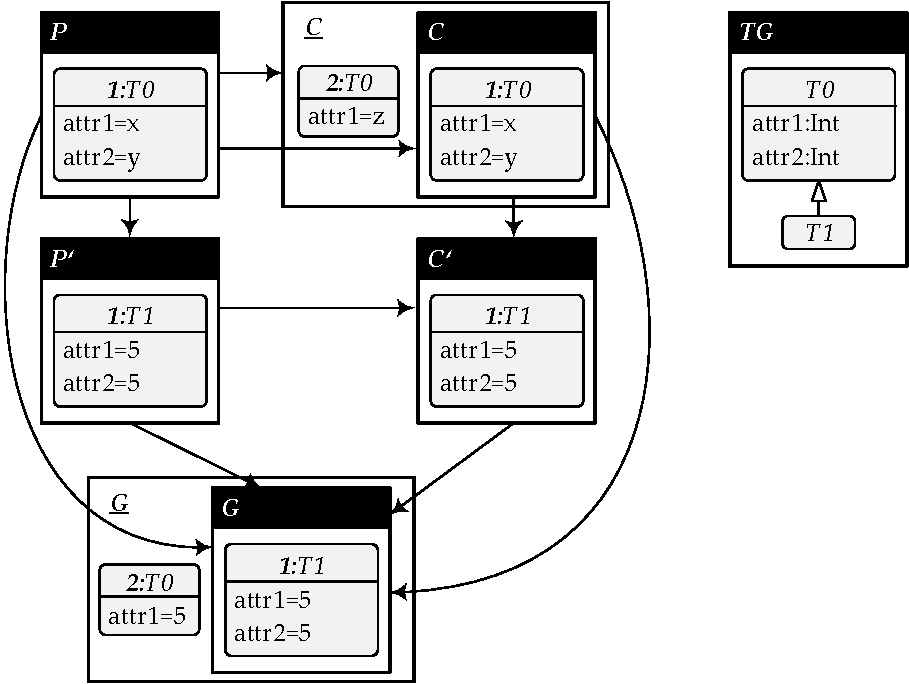
\includegraphics[width=.75\textwidth]{img/gen_intro/ac_schema.pdf}};
\fill (-2.5,2.55) node[inner sep=1pt] (B) {$a$};
\fill (-6.25,0) node[inner sep=1pt] (C) {$p \in \morO$};
\fill (3.2,0) node[inner sep=1pt] (D) {$\not\exists q \in \M$};
\fill (-2.5,.7) node[inner sep=1pt] (E) {$a'$};
\fill (-4.6,1.5) node[inner sep=1pt] (F) {$e \in \E$};
\fill (-4.1,-1.35) node[inner sep=1pt] (G) {$m \in \M$};
\fill (.4,1.5) node[inner sep=1pt] (H) {$e'$};
\fill (-.5,-1.35) node[inner sep=1pt] (I) {$\exists q' \in \M$};
\fill (-2.5,3.5) node[inner sep=1pt] (B2) {$\underline{a}$};
\end{tikzpicture}
\end{center}
\caption{Non-Satisfiability and Instance of Condition $\ac_P=\exists(a\colon P \to C \in \M,\true)$ along $\morO$-matches (left) \& Type Graph $\TG$ (right)}
\label{fig:sec-gc-gc:ac_schema}
\end{figure}

According to \cref{def:condition-satisfaction}, match morphisms $p$ are in $\morO$ but morphisms $q$ are in $\M$ for standard satisfiability of conditions.
Therefore according to \cref{sec-gt-M-adh,rem:sec-gt-M-adh:agraphs_atgi} in $(\AGraphs_\ATGI,\M)$, match morphisms $p$ may be non-injective on the data part $p_D$ and may refine node types along a node type inheritance relation whereas morphisms $q$ are isomorphisms on the data part $q_D$ and are type strict.
More specifically, in category $(\AGraphs_\ATGI,\M)$, conditions $\ac_P$ are often attributed via the $\DSIG$-term algebra $T_\DSIG(X)$ over variables $X$ whereas graphs $G$ are attributed via a concrete $\DSIG$-algebra $D_G$.
In most cases $T_\DSIG(X)$ is not isomorphic to $D_G$, since, different terms in $T_\DSIG(X)$ may be evaluated to the same concrete value in $D_G$, and therefore, $q \in \M$ does not exist.
Thus, a condition $\ac_P$ in $\M$-normal form may be non-satisfiable by $p$ although the condition seems to be a tautology as shown in \cref{fig:sec-gc-gc:ac_schema} where $p$ identifies variables $x$ and $y$ with value $5$ as well as refines type $T_0$ to $T_1$ along the inheritance relation in type graph $\TG$ and there does not exist $q \in \M$ with $q \circ a=p$.
Therefore, according to \cref{def:AC-schemata}, we use the concept of an AC-schema, which interprets a constraint $\ac_P$ as the disjunction of its possible instances $\Inst(\ac_P)$ which may occur in a graph.
Based on the merge construction over extremal $\E$-morphisms w.r.t. $\M$ in \cref{def:merge morphism}, the instances $\Inst(\ac_P)$ subsume all possible type refinements and identifications of data values along match morphisms (cf. \cref{def:sec-gc-gc:cond_inst}).
Since, according to \cref{rem:sec-gc-gc:schemata}, the satisfaction of an AC-schema by match $p \in \morO$ coincides with the satisfaction of the corresponding instance in the schema by $m \in \M$ that is derived by the $\E$-$\M$ factorisation of $p$, this allows us to use AC-schemata as a compact notation and to focus on $\M$-matches while leaving the possible type refinements and identifications of data values implicit.
For example, $(e,\exists(a'\colon P' \to C',\true))$ is an instance of $\ac_P$ in \cref{fig:sec-gc-gc:ac_schema} (the identification of variables $x$ and $y$ as well as the type refinement from $T_0$ to $T_1$ is transferred to the instance), $m \circ e=p$ is an $\E$-$\M$ factorisation of $p$ and furthermore, there exists $q' \in \M$ with $q' \circ a'=m$ (i.e., $m$ satisfies the instance) and therefore, $p$ satisfies the AC-schema of $\ac_P$.
Furthermore, in \cref{th:sec-gc-gc:rel_sat_ac_schema} we show that the standard satisfiability of an AC-schema coincides with the $\morO$-satisfiability of the underlying condition.
This allows an interpretation of conditions via $\morO$-matches and $\morO$-satisfiability from a user point of view while an interpretation via the standard satisfiability of AC-schemata with $\M$-matches is used to prove technical results.

Intuitively, the merge construction transfers the identifications of data values and type refinements along the given morphism $b \colon P \to P'$ to $b' \colon C \to C'$ by respecting the identifications and type refinements along $a\colon P \to C$.
Additionally, it allows for type refinements of elements and identifications of data elements that are in $C$ but not in $P$. 

\begin{definition}[Merge over Morphism (Def. 5.5 in \cite{FAGT2})]
\label{def:merge morphism}
\index{morphism!merge over morphism}
Given a condition $\ac$ over $P$ and a morphism $b: P \rightarrow P'$, then \emph{$\Merge(b,\ac)$ is a condition over $P'$} defined by
\begin{itemize}
\item $\Merge(b,\ac) = \true$ if $\ac = \true$,
\pichskip{5pt}
\parpic[r]{
\begin{tikzpicture}[]
\fill (.5,1.7) node[inner sep=1pt] (P) {$P$};
\fill (2.5,1.7) node[inner sep=1pt] (C) {$C$};
\fill (0.5,-.5) node[inner sep=1pt] (P') {$P'$};
\fill (2.5,-.5) node[inner sep=1pt] (C') {$C'$};
\fill (1.5,.6) node[inner sep=1pt] (N) {$(1)$};
\fill (3.1,1.7) node [isosceles triangle, fill=gray!25,draw,shape border rotate=180,minimum width=0.4cm, inner sep=1pt] (t) {};
\fill (-.1,1.7) node [isosceles triangle, fill=gray!25,draw,minimum width=0.4cm, inner sep=1pt] (t) {};
\fill (-.1,-.5) node [isosceles triangle, fill=gray!25,draw,minimum width=0.4cm, inner sep=1pt] (t) {};
\fill (3.1,-.5) node [isosceles triangle, fill=gray!25,draw,shape border rotate=180,minimum width=0.4cm, inner sep=1pt] (t) {};
\fill (-.5,1.7) node[inner sep=1pt] {$\ac$};
\fill (0.2,-.9) node[inner sep=1pt] {$\Merge(b,\ac)$};
\fill (3.5,1.7) node[inner sep=1pt] {$\ac'$};
\fill (2.7,-.9) node[inner sep=1pt] {$\Merge(b',\ac')$};
%
{
\pgfsetarrowsend{latex}
\draw (P) -> node[above,inner sep=1pt]{$\scriptstyle{a}$} (C);
\draw (P) -> node[left,inner sep=1pt]{$\scriptstyle{b}$} (P');
\pgfsetarrows{right hook-latex}
\draw (P') -> node[above,inner sep=1pt]{$\scriptstyle{a' \in \M}$} (C');
\pgfsetarrows{*-latex}
\draw (C) -> node[right,inner sep=1pt]{$\scriptstyle{b' \in \morO}$} (C');
}
\end{tikzpicture}
}
\item $\Merge(b,\ac) = \vee_{(a',b')\in{\cal F}} \exists(a',\Merge(b',\ac'))$ if $\ac = \exists(a,\ac')$ and ${\cal F} = \{(a',b') \mid a' \in \M \wedge b' \in \morO \wedge (1) \n{ commutes } \wedge (a',b') \n{ are } \n{jointly epimorphic}\}$,
\item $\Merge(b,\ac) = \neg \Merge(b,\ac')$ if $\ac = \neg \ac'$,
\item $\Merge(b,\ac) = \wedge_{i \in{I}} \Merge(b,\ac_i)$ if $\ac = \wedge_{i \in {I}} \ac_i$, or
\end{itemize}
\vspace*{-11pt}
\begin{itemize}
\item $\Merge(b,\ac) = \vee_{i \in{I}} \Merge(b,\ac_i)$ if $\ac = \vee_{i \in {I}} \ac_i$.
\envEndMarker
\end{itemize}
\end{definition}

\begin{remark}
\label{rem:mom}
In $(\AGraphs_\ATGI,\M)$, note that if morphism $a$ identifies elements of $P$ or refines types in $P$ that are not identified or not refined to equal or finer types by morphism $b$, respectively, then $(1)$ cannot be constructed, since, it is required that $a' \in \M$ while $(1)$ commutes, and the merge construction returns $\false$ (an empty disjunction over $(a',b')\in{\cal F}$).
Analogously, if morphism $b$ identifies graph elements of $P$ that are not identified by morphism $a$, then $(1)$ cannot be constructed and $\false$ is returned, since, it is required that $b' \in \morO$ while $(1)$ commutes.
For a characterisation of $\M$- and $\morO$-morphisms in $(\AGraphs_\ATGI,\M)$ we refer to \cref{sec-gt-M-adh,rem:sec-gt-M-adh:agraphs_atgi}.
\envEndMarker
\end{remark}

\begin{definition}[Instances of Conditions]
\label{def:sec-gc-gc:cond_inst}
Given a condition $\ac_P$ over $P$ with $\mor{E}_P = \{e \in \mor{E}\ |\ \dom(e)=P\}$ being the set of all extremal $\E$-morphisms w.r.t. $\M$ with domain $P$.
The \emph{instances of $\ac_P$}\index{graph condition!instance} are given by $\Inst(\ac_P)=\bigcup_{f \in \mor{E}_P}\{(f,\Merge(f,\ac_P))\}$.
Given a set of conditions $C$, then the instances of $C$ are given by $\Inst(C)=\bigcup_{\ac \in C}(\Inst(\ac))$.
\envEndMarker
\end{definition}

\begin{remark}[Instances in $\M$-normal Form]
\label{rem:sec-gc-gc:inst_m_norm_form}
Note that the conditions in instances are in $\M$-normal form by merge construction.
\envEndMarker
\end{remark}

\begin{definition}[AC-schema (Def. 5.6 in \cite{FAGT2})]
\label[definition]{def:AC-schemata}
Given a condition $\ac_P$ over $P$, then \emph{the AC-schema $\ol{\ac}_P$ of $\ac_P$}\index{graph condition!AC-schema} is a condition over $P$ given by  $\ol{\ac}_P = \bigvee_{(f,\ac) \in \Inst(\ac_P)} \exists(f,\ac)$.
For $\ac_P=\true$, $\ol{\ac}_P=\true$.
\envEndMarker
\end{definition}

\vspace*{-10pt}
\pichskip{5pt}
\parpic[r]{
\begin{tikzpicture}[]
\fill (.5,1.3) node[inner sep=1pt] (P) {$P$};
\fill (2,.5) node[inner sep=1pt] (P') {$P'$};
\fill (3.5,1.3) node[inner sep=1pt] (G) {$G$};
\fill (-.1,1.3) node [isosceles triangle, fill=gray!25,draw,minimum width=0.4cm, inner sep=1pt] (t) {};
\fill (1.4,.5) node [isosceles triangle, fill=gray!25,draw,minimum width=0.4cm, inner sep=1pt] (t) {};
\fill (-.6,1.3) node[inner sep=1pt] {$\ol{\ac}_P$};
\fill (.1,0.5) node[inner sep=1pt] {$\Merge(e,\ac_P)$};
%
{
\pgfsetarrows{*-latex}
\draw (P) -> node[above,inner sep=1pt]{$\scriptstyle{p}$} (G);
\pgfsetarrows{->>}
\draw (P) -> node[below left,inner sep=1pt]{$\scriptstyle{e}$} (P');
\pgfsetarrows{right hook-latex}
\draw (P') -> node[below right,inner sep=1pt]{$\scriptstyle{m}$} (G);
}
\end{tikzpicture}}
\vspace*{-10pt}
\begin{remark}[AC-schema satisfaction (Fact 5.8 in \cite{FAGT2})]
\label{rem:sec-gc-gc:schemata}
\index{graph condition!AC-schema!satisfaction}
Given an AC-schema $\ol{\ac}_P$ of condition $\ac_P$ over $P$ and a morphism $p \colon P \to G \in \morO$ with an extremal $\E$-$\M$-factorisation $m \circ e = p$, then $p \models \ol{\ac}_P$ if and only if  $m \models \Merge(e,\ac_P)$ with $(e,\Merge(e,\ac_P)) \in \Inst(\ac_P)$.
Note that the satisfaction of conditions by morphisms in \cref{sec-gt-gc,def:condition-satisfaction} is defined based on $\morO$-morphisms.
However, $m \in \morO$ by $m \in \M$ in $(\AGraphs_\ATGI,\M)$ (cf. \cref{sec-gt-M-adh,rem:sec-gt-M-adh:agraphs_atgi}).
\envEndMarker
\end{remark}

Note that by \cref{def:AC-schemata}, the AC-schema $\ol{\ac}_P$ of a constraint $\ac_P$ over $P$ is again a constraint over $P$.
However, the satisfaction of AC-schemata by objects cannot be directly defined by \cref{rem:sec-gc-gc:init_gen_sat}.
For example, constraint $\neg\ac_P$ in \cref{fig:sec-gc-gc:ac_schema} seems to be a contradiction with $G \not\models \neg\ac_P$ but $G \models \neg\ac_P$ if both algebras of $G$ and $\neg\ac_P$ are not isomorphic, i.e., $p\colon P \to G \in \M$ does not exist (cf. \cref{sec-gt-M-adh,rem:sec-gt-M-adh:agraphs_atgi}).
Therefore, based on \cref{rem:sec-gc-gc:init_gen_sat} the satisfaction of AC-schemata is defined as follows.

\begin{definition}[Initial \& General Satisfaction of AC-schemata]
\label{rem:sec-gc-gc:init_gen_sat_ac_schema}
\index{graph constraint!AC-schema!initial satisfaction}
\index{graph constraint!AC-schema!general satisfaction}
\emph{An object $G$ initially satisfies AC-schema $\ol{\ac}_P$} of constraint $\ac_P$ over $P$, if $\exists p\colon P \to G \in \morO$ such that $p \models \ol{\ac}_P$.
\emph{An object $G$ generally satisfies $\ol{\ac}_P$}, if $\forall p\colon P \to G \in \morO$ it holds that $p \models \ol{\ac}_P$.
By \cref{rem:sec-gc-gc:schemata}, in $\M$-adhesive categories with extremal $\E$-$\M$ factorisations, $G$ initially satisfies $\ol{\ac}_P$ if and only if $\exists$ instance $(e\colon P \to P',\Merge(e,\ac_P)) \in \Inst(\ac_P)$ of $\ac_P$ such that $G \stackrel{I}{\models} \Merge(e,\ac_P)$.
Analogously, $G$ generally satisfies $\ol{\ac}_P$ if and only if $\forall$ instances $(e\colon P \to P',\Merge(e,\ac_P)) \in \Inst(\ac_P)$ it holds that $G \models \Merge(e,\ac_P)$.
For initial and general satisfaction of constraints $\Merge(e,\ac_P)$, we refer to \cref{def:constr_sat,rem:sec-gc-gc:init_gen_sat}.
\envEndMarker
\end{definition}

\begin{remark}[Data in Constraints and Application Conditions]
\label{rem:sec-gc-gc:data_cond}
Consider condition $\ac'_P=\exists(\underline{a}\colon P \to \underline{C},\true)$ in \cref{fig:sec-gc-gc:ac_schema} with $P,\underline{C}$ being attributed graphs and which claims that there is an additional \code{:T0} node with attribute \code{attr1} of value \code{z}.
Assume that $P$ contains a variable \code{z'} in its algebra that is mapped to variable \code{z} in $\underline{C}$ along morphism $\underline{a}$, then the interpretation of $\ac'_P$ according to \cref{rem:sec-gc-gc:init_gen_sat_ac_schema} may be misleading, e.g., in contrast to the intended result, $\underline{G}$ does not generally satisfy the AC-schema $\ol{\ac}'_P$ of constraint $\ac'_P$.
This is due to the fact that the mapping of \code{z} along $\underline{q}\colon \underline{C} \to \underline{G} \in \morO$ is prescribed by the mapping of \code{z'} along match $\underline{p}\colon P \to \underline{G} \in \morO$ in order to obtain $\underline{q} \circ \underline{a}=\underline{p}$ (cf. \cref{th:sec-gc-gc:rel_sat_ac_schema}).
By \cref{rem:sec-gc-gc:init_gen_sat_ac_schema}, for general satisfaction all matches $\underline{p}\colon P \to \underline{G} \in \morO$ are considered, i.e., \code{z'} and therefore also \code{z} may be mapped to the same value than \code{x} or \code{y} (i.e., value \code{5} for the example) but also to any other value along $\underline{p}$ and $\underline{q}$, respectively.
Thus, more precisely, for general satisfaction and graphs $\underline{G}$ that allow different values for variables \code{x}, \code{y} and \code{z}, $\ac'_P$ claims that there are additional \code{:T0} nodes, one with attribute \code{attr1} of value \code{z} that equals to \code{x}, one with attribute \code{attr1} of value \code{z} that equals to \code{y} and one with attribute \code{attr1} of value \code{z} that differs from \code{x} and \code{y}.
The same situation arises for variables that are not used as attribute values in attributed premise and conclusion graphs of conditions but that are non-injectively mapped along the internal morphisms of conditions, since, for matches $\underline{p}$ that are injective on these variables, the corresponding $\underline{q}$-morphism with $\underline{q} \circ \underline{a}=\underline{p}$ does not exist. 
Therefore, for conditions $\ac$ over attributed graphs we generally assume that for all internal morphisms $a\colon P \to C$ in $\ac$ it is true that all variables that are used as attribute values in $C$ but not in $P$ are not in the image of $a$.
Furthermore, all variables in $P$ that are not used as attribute values are injectively mapped along $a$.
Under this general assumption for constraint $\ac'_P$, graph $\underline{G}$ both initially and generally satisfies $\ol{\ac}'_P$.
\envEndMarker
\end{remark}

According to \cref{prop:sec-gc-gc:rel_sat_cond_ac}, for $\M$-matches and the case of category $(\AGraphs_\ATGI,\M)$ (and underlying categories $(\Graphs,\M)$ and $(\Graphs_\TG,\M)$), the interpretation of a condition $\ac_P$ that is type strict via the standard satisfiability of its AC-schema coincides with the standard satisfiability of $\ac_P$ itself.
According to \cref{def:sec-gc-gc:cond_type_strict}, a condition $\ac_P$ over $P$ is type strict, if it is in $\M$-normal form and furthermore, the types of all nodes in conclusions that are not in premise $P$ cannot be refined along morphisms.
Therefore, for $\M$-matches and type strict conditions, the direct interpretation of conditions is equivalent to their interpretation via AC-schemata.
This may not hold for general $\morO$-matches and for conditions that are not type strict.
However, \cref{th:sec-gc-gc:rel_sat_ac_schema} shows for $(\AGraphs_\ATGI,\M)$ and underlying categories that the standard satisfiability of an AC-schema coincides with the $\morO$-satisfiability of the underlying condition.

\begin{definition}[Type Strict Condition]
\label{def:sec-gc-gc:cond_type_strict}
In $(\AGraphs_\ATGI,\M)$, \emph{a condition $\ac_P$ over $P$ is type strict}\index{graph condition!type strict}, if $\ac_P$ is in $\M$-normal form and for all morphisms $a\colon P \to C$ in $\ac_P$ with domain $P$ it holds that for all nodes $n \in V_G^C \setminus a_{G,V_G}(V_G^P)$ that are in $C$ but not in $P$, node type $\type_C(n)$ does not have sub-types in the inheritance relation of type graph $\ATGI$ and therefore, cannot be refined along morphisms.
\envEndMarker
\end{definition}

\begin{proposition}[Relationship between Satisfiability of Conditions and AC-Schemata]
\label{prop:sec-gc-gc:rel_sat_cond_ac}
\index{graph constraint!AC-schema!satisfaction (relationship to conditions I)}
In $(\AGraphs_\ATGI,\M)$, given a type strict condition $\ac_P$ over $P$, its AC-schema $\ol{\ac}_P$ and a match $p:P \to G \in \M$.
Then, $p \models \ac_P$ if and only if $p \models \ol{\ac}_P$.
\envEndMarker
\end{proposition}

\begin{proof}
The proof is presented in \cref{sec-proofs:prop:sec-gc-gc:rel_sat_cond_ac}.
\end{proof}

\begin{proposition}[Relationship between Standard- and $\morO$-Satisfiability of Conditions]
\label{th:sec-gc-gc:rel_sat_ac_schema}
\index{graph constraint!AC-schema!satisfaction (relationship to conditions II)}
In $(\AGraphs_\ATGI,\M)$, given a condition $\ac_P$ over $P$, its AC-schema $\ol{\ac}_P$ and a match $p\colon P \to G \in \morO$.
Then, $p \models_{\morO} \ac_P$ if and only if $p \models \ol{\ac}_P$.
\envEndMarker
\end{proposition}

\begin{proof}
The proof is presented in \cref{sec-proofs:th:sec-gc-gc:rel_sat_ac_schema}.
\end{proof}

\paragraph*{General Assumption}
Note that we interpret conditions by AC-schemata that are formed over (extremal) $\E$-morphisms and their satisfaction can be defined based on (extremal) $\E$-$\M$ factorisations by \cref{rem:sec-gc-gc:schemata}.
Therefore, in addition to the general assumption from \cref{sec-gt-M-adh}, we assume $\M$-adhesive categories with unique (extremal) $\E$-$\M$ factorisation.
Furthermore, we assume that all application conditions and graph constraints are interpreted via their AC-schemata according to \cref{def:AC-schemata}, if not made explicit.
Moreover, we generally assume the assumption from \cref{rem:sec-gc-gc:data_cond} for constraints.